\documentclass[12pt]{beamer} 
\usepackage{times}
\usepackage[]{algorithm2e}
%\SetKw{def}{def}
%\SetKw{To}{to} 
%\SetKw{Othera}{other}
%\SetKw{Become}{become}

\usepackage[T1]{fontenc} % bedre orddeling og ofte påkrævet at
\usepackage[utf8]{inputenc} % eller utf8 eller ansinew eller ...
\usepackage[english, danish]{babel} %direktiv til at bruge det danske sprog
\usepackage{graphicx} % pakke til inklusion af grafik
 
\renewcommand\danishhyphenmins{22} % bedre orddeling
\addto\captionsdanish{
\renewcommand\contentsname{Indholdsfortegnelse}
\renewcommand\appendixname{Appendix}
}
\selectlanguage{danish}
 
\usepackage[]{booktabs}
\usepackage{listings}
 \lstset{ 
         basicstyle=\tiny\ttfamily, % Standardschrift
         numbers=left,               % Ort der Zeilennummern
         numberstyle=\tiny,          % Stil der Zeilennummern
         stepnumber=2,               % Abstand zwischen den Zeilennummern
         numbersep=5pt,              % Abstand der Nummern zum Text
         tabsize=2,                  % Groesse von Tabs
         extendedchars=true,         %
         breaklines=false,            % Zeilen werden Umgebrochen
         keywordstyle=\color{red},
                frame=b,         
         keywordstyle=[1]\textbf,    % Stil der Keywords
         keywordstyle=[2]\textbf,    %
         keywordstyle=[3]\textbf,    %
         keywordstyle=[4]\textbf,   %\sqrt{\sqrt{}} %
         stringstyle=\color{black}\ttfamily, % Farbe der String
         showspaces=false,           % Leerzeichen anzeigen ?
         showtabs=false,             % Tabs anzeigen ?
         xleftmargin=17pt,
         framexleftmargin=17pt,
         framexrightmargin=5pt,
         framexbottommargin=4pt,
         %backgroundcolor=\color{lightgray},
         showstringspaces=false      % Leerzeichen in Strings anzeigen ?        
 }

 \lstloadlanguages{% Check Dokumentation for further languages ...
         [Visual]Basic,
         Pascal,
         C,
         C++,
         XML,
         HTML,
         PYTHON,
 }
\lstset{language=Python}
\lstset{emph={@process, @choise,choice, Alternation, Skip,Timeout,Parallel,Sequence, Spawn,@io,ChannelPoisonException, ChannelRetireException},emphstyle=\underbar}

\newcommand\mc[1]{\multicolumn{1}{c}{\textbf {#1}}} % sparer plads


% A few keywords to use in pseudocode
% You should also probably read the algorithm2e -documentation more than I did.

\usetheme[nat,dk,style=simple]{Frederiksberg}% Beamer theme v 3.0
%\mode<presentation>
%{
%\usetheme{Rochester}% Beamer theme v 3.0
%\usecolortheme{whale}
%   \setbeamercovered{transparent}
%   \definecolor{beamer@tkkblue}{HTML}{0041AD}
%   \setbeamercolor{structure}{fg=beamer@tkkblue}
%} 
\title
{Timed PyCSP}
%\subtitle
%{Specialeforsvar}
\institute
{Datalogisk Institut \\ Københavns Universitet}
\author
{Simon Bognolo}
\date
{5 juli 2010}


\begin{document}

\frame[plain]\titlepage
 
\begin{frame}
  \frametitle{Oversigt}
  \tableofcontents
\end{frame}

\section{Mål}
\begin{frame}
  \frametitle{Praktisk anvendelig implementering af tid i CSP}
  \begin{itemize}
	\item Tilbyde en ensartet håndtering af tid i PyCSP
	\item Let at anvende
	\item Brugbar
	\item håndtere tilstande tilknyttet tid, som ikke direkte er relateret til problemet
  \end{itemize}
\end{frame}

\begin{frame}
  \frametitle{Scheduler i PyCSP}
  \begin{itemize}
	\item er også en brugertråd
	\item ingen tvungen kontekstskift
	\item Timeouts og timers listen.
  \end{itemize}
\end{frame}

\begin{frame}
  \frametitle{Gennemgang af scheduler}
  \includegraphics[scale=0.9]{pycsp-scheduler} 
\end{frame}

\section{DES}
\begin{frame}
  \frametitle{DES}
Eksempel : MIG 
\end{frame}


\begin{frame}
\frametitle{Implementering}
  \begin{itemize}   
	\item Udvide scheduler
	\item Håndtering af køer
  \end{itemize}
\end{frame}
 
\begin{frame}
\frametitle{Udvidelsen af scheduler}
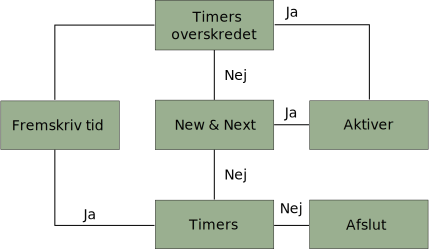
\includegraphics[scale=0.9]{des-scheduler} 
\end{frame}

 \subsection{Resultater}
\begin{frame}[fragile]
  \frametitle{Greenlets-version}
\begin{lstlisting}
@process
def Generator(i,number,meanTBA, meanWT,
              customerWRITER,barrierWRITER,barrierREADER):
  t_event = 0
  time = 0
  numberInserted = 0
  while numberInserted<number:
    if t_event<=time:
      customerWRITER(Customer(name = "Customer%d:%02d"%
                     (i,numberInserted),meanWT=meanWT))
      t_event = time + round(expovariate(1/meanTBA))
      numberInserted+=1
    barrierWRITER(0)
    barrierREADER()
    time+=1
  retire(customerWRITER)
  try:
    while True:
      barrierWRITER(0)
      barrierREADER()
      time +=1
  except ChannelPoisonException: 
    return
\end{lstlisting}
\end{frame}

\begin{frame}[fragile]
  \frametitle{DES-version}
\begin{lstlisting}
@process
def Generator(i,number,meanTBA, meanWT, customerWRITER):
  for numberInserted in range(number):
    customerWRITER(Customer(name = "Customer%d:%02d"%(i,numberInserted),
                            meanWT = meanWT))
    Wait(expovariate(1/meanTBA))
  retire(customerWRITER)
\end{lstlisting}
\end{frame}

\section{RTP}
\begin{frame}
  \frametitle{RTP eksempel}
  \begin{itemize}   
    \item GRIS
  \end{itemize}
\end{frame}

\begin{frame}
  \frametitle{RTP scheduler}
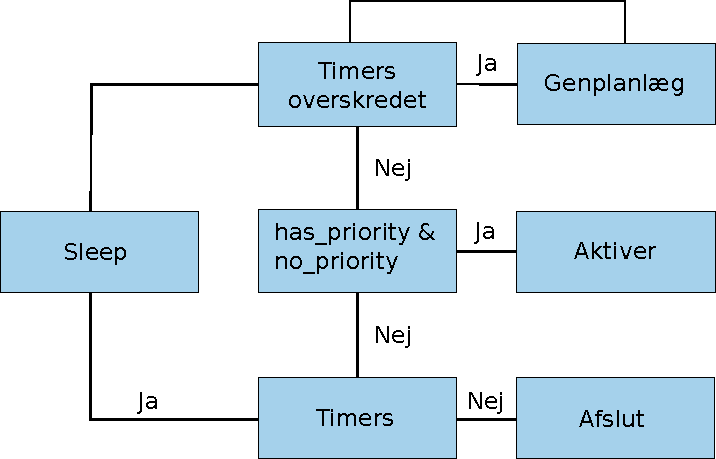
\includegraphics[scale=0.9]{rtp-scheduler} 
\end{frame}



%	\item Deadline exception
%prioriteter



\begin{frame}
  \frametitle{Prioritetsnedarvning}
\begin{itemize}
	\item Proces kalder Write() 
	\item Kanalen gennemløber liste af Readers
	\item Såfremt ingen readers er klar foretages prioritetsnedarvning
	\item Hver reader arver writerprocessens prioritet 
	\item Såfremt nedarvning medfører en forbedret prioritet genscheduleres processen
	\item Når en reader er klar gennemføres kommunikation
	\item Readers sættes tilbage til deres forrige prioritet
  \end{itemize}
\end{frame}

\begin{frame}
	\frametitle{Kommunikation}
	\begin{itemize}
		\item Udfordring ved Any-to-Any Kanaler 
	 	\item Alternation
	\end{itemize} 
\end{frame} 

\subsection{Resultater}
\begin{frame}
  	\frametitle{RTP resultater}
	\tiny 
	\begin{table}[htbp]
		\centering
		\begin{tabular}{lcccc}
		   	\toprule
		    \mc{Version}&\mc{Tid i dummyproces(s)}&\mc{SA.}& \mc{Succesrate (\%)}&\mc{SA.}\\
		    \midrule
		    Greenlets         & 1.29 & 0.61 & 13 & 2  \\
		    RTP u. prioritet  & 1.05 & 0.28 & 24 & 6  \\
		    RTP m. prioritet  & 0.74 & 0.34 & 42 & 13 \\
		    \bottomrule
		\end{tabular}
		\caption[]{\tiny 10 * 100 grise køres igennem procesnetværket. Samtidigt køres en dummyproces.}
	\end{table}
\end{frame} 

\section{Fremtidigt arbejde}
\begin{frame}
  	\frametitle{Fremtidigt arbejde}
\begin{itemize}
\item DES
	\begin{itemize}
	\item Dynamisk køskifte
	\item Reservering af flere ressurcer
	\item Stopkriterium
	\item Parallelisering
	\end{itemize}
\item RTP
	\begin{itemize}
	\item Estimater for udførselstid
	\item Samarbejde med operativsystemet
	\item Forskellige typer deadlines
	\end{itemize}
\end{itemize}
\end{frame}
 




%\section*{Vi mangler at snakke om:}
%\begin{frame}
%  \frametitle{Blandede noter}
%  \begin{itemize}
%    \item Barrierer
%	\item shared memory
%  \end{itemize}  
%\end{frame}

%\begin{frame}
%  \frametitle{Blandede noter}
%  \begin{itemize}
%    \item Sætte begrænsning på kommunikation ifh. til tid.
%    \item MOTIVATION!
%  \end{itemize}
%\end{frame}


%\section*{Noter fra tavlen}
%\begin{frame}
%  \frametitle{Blandede noter}
%  \begin{itemize}
%    \item Håndtering af tilstande, som ikke direkter er relateret til problemet.
%    \item Sætte begrænsning på kommunikation ifh. til tid.
%    \item MOTIVATION!
%  \end{itemize}
%\end{frame}

%\begin{frame}
%  \frametitle{Anvendelse}
%  \begin{itemize}
%	\item MIG
%	\item GRISE
%	\item Fabrik
%	\item Trafik
%	\item vejr, hav forudsigelser mv,
%  \end{itemize}
%\end{frame}


%\begin{frame}
%  \frametitle{TID}
%  \begin{itemize}
%	\item Forventet mål 3-5 min
%	\item Tidsmodel
%	\item DES 10 min.
%	\item RTP 5 min.
%	\item Finale 5 min.
%  \end{itemize}
%\end{frame}

\end{document}

 
